\begin{landscape}
\begingroup
\fontsize{10}{13}\selectfont
\fancyhead[L]{\small NACHLASS UND BRIEFWECHSEL}
\renewcommand{\headrulewidth}{0pt}
\par\medskip
\pdfbookmark[2]{Nachlass VII [3]}{pallas-VII-letters3}
\begin{center}[3.]\par\medskip
\textsc{Gauss} an \textsc{Encke}, Göttingen, 7. November 1816.
\end{center}
\par\noindent\hspace*{\parindent}Ihrem freundlichen Angebot zufolge .\ .\ .\ .\ .\ übersende ich Ihnen hier
heute einige Rechnungen für die Pallasstörungen. Zur Erläuterung bemerke
ich zuerst, was noch zu tun ist. Es gibt drei Arten von Operationen:
\par\noindent\hspace*{\parindent}Die \textls[100]{erste Operation} ist bereits ganz abgeschlossen, sodass es sich erübrigt,
sie hier näher zu beschreiben.
\par\noindent\hspace*{\parindent}\textls[100]{Zweite Operation} nenne ich die Berechnung von 24 Werten einer
Funktion der Form
\[
\odot)\qquad
\begin{aligned}
&a+a'\cos x+a''\cos2x+a'''\cos3x+\text{etc.}+a^{\mathrm{XII}}\cos12x\\
&\quad+b'\sin x+b''\sin2x+b'''\sin3x+\text{etc.}+b^{\mathrm{XII}}\sin12x
\end{aligned}
\]
\noindent für \(x=0^0\), \(x=15^0\), \(x=30^0\) usw. bis \(x=345^0\). Diese Operation müsste
insgesamt 126-mal ausgeführt werden, davon stehen noch 62 aus.
\par\noindent\hspace*{\parindent}\textls[100]{Dritte Operation} nenne ich die 24-malige Bestimmung von \(\log r\) und \(\varphi\) aus
\[
\begin{aligned}
r\cos\varphi&=P\\
r\sin\varphi&=Q
\end{aligned}
\]
\SourceLeaf{575}
\noindent wobei \(P\) und \(Q\) gegebene (jeweils aus der Form \(\odot\) berechnete) Größen
sind. Diese Operation war insgesamt 60-mal auszuführen. Es fehlen jetzt noch 48.
\par\noindent\hspace*{\parindent}Heute schicke ich Ihnen auf 8 kleinen Blättern die Daten, um 8-mal die dritte
Operation auszuführen. Jedes \(P\) ergibt sich aus den unten stehenden Zahlen
der Seite, über der \(\sin A\) steht. Jedes \(Q\) ergibt sich aus den Zahlen der anderen Seite,
über der \(\cos A\) steht, und zwar auf folgende Weise. Jedes \(P\) besteht aus zwei Teilen
(die sich aus den Kosinus- beziehungsweise Sinusgliedern ergeben). Diese
zwei Teile finden Sie unmittelbar für 13 Werte in
dieser Reihenfolge angegeben
\providecommand{\VIIthreeStars}[1]{\begin{array}{@{}c@{}}\ast\\\ast\end{array}\;#1}
\begingroup\small
\[
\begin{aligned}
&\begin{array}{c|c|c|c|c|c|c}
\VIIthreeStars{0^0}&\VIIthreeStars{30^0}&\VIIthreeStars{60^0}&\VIIthreeStars{90^0}&\VIIthreeStars{120^0}&\VIIthreeStars{150^0}&\VIIthreeStars{180^0}
\end{array}\\[1ex]
&\begin{array}{c|c|c|c|c|c|}
\VIIthreeStars{15^0}&\VIIthreeStars{45^0}&\VIIthreeStars{75^0}&\VIIthreeStars{105^0}&\VIIthreeStars{135^0}&\VIIthreeStars{165^0}
\end{array}
\end{aligned}
\]
\endgroup
\par\noindent\hspace*{\parindent}Anschließend geht man in derselben Reihenfolge rückwärts, wobei man den zweiten
(Sinus-)Teil stets mit entgegengesetztem Vorzeichen nimmt. So ergibt sich also z. B.
auf dem ersten Blatt für
\[
\begin{array}{r|r|r}
x&P&Q\\
0^0&+39{,}5723&-24{,}3180\\
15^0&+18{,}4497&-17{,}9717\\
30^0&-1{,}5499&-18{,}3889\\
\vdots&\vdots&\vdots\\
180^0&-6{,}8889&-39{,}1004\\
195^0&-5{,}3849&-40{,}6708\\
210^0&-2{,}6665&-42{,}6184\\
\vdots&\vdots&\vdots
\end{array}
\]
\par\noindent Eine vollständige Rechnung der zweiten Operation führe ich auf einer einzigen Oktavseite
in dieser Form aus, und zwar für
\begingroup\renewcommand{\arraystretch}{1.8}\setlength{\tabcolsep}{13pt}
\begin{center}
\begin{tabular}{|c|c|c|c|c|c|}
\hline
\(0^0\)&\(15^0\)&\(30^0\)&\(45^0\)&\(60^0\)&\(75^0\)\\\hline
\(90^0\)&\(105^0\)&usw.&&&\\\hline
\rule{0pt}{1.8em}&&&&&\\\hline
\rule{0pt}{1.8em}&&&&&\\\hline
\end{tabular}
\end{center}\endgroup
\SourceLeaf{576}
\par\noindent Das erste Quadrat sähe nach meiner Art zu rechnen so aus:
\begin{center}
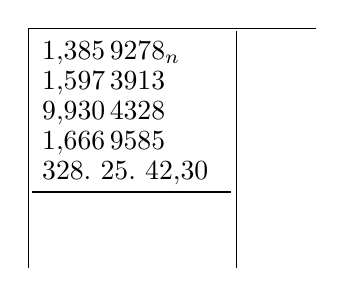
\begin{tikzpicture}[x=1cm,y=1cm]
\draw (0,-.75)--(0,2.30)--(3.65,2.30);
\draw (2.65,-.75)--(2.65,2.27);
\draw (.05,.22)--(2.58,.22);
\node[anchor=west,inner sep=0pt] at (.17,1.98) {\(1{,}385\,9278_n\)};
\node[anchor=west,inner sep=0pt] at (.17,1.60) {\(1{,}597\,3913\)};
\node[anchor=west,inner sep=0pt] at (.17,1.22) {\(9{,}930\,4328\)};
\node[anchor=west,inner sep=0pt] at (.17,.84) {\(1{,}666\,9585\)};
\node[anchor=west,inner sep=0pt] at (.17,.46) {\(328.\ 25.\ 42{,}30\)};
\end{tikzpicture}
\end{center}
\par\noindent Ich lasse nämlich \(\log\operatorname{tang}\varphi\) weg. Falls es für Sie
so unpraktisch ist, schreiben Sie es dazu.
Dann bitte ich Sie um die vollständige Rechnung,
damit ich sie leichter vergleichen kann, falls sich irgendwo
Unterschiede zeigen sollten. Dagegen brauchen Sie
nicht mit übertriebener Sorgfalt zu rechnen. Die Ihnen jetzt aufgegebenen Rechnungen werden also 4 Oktavblätter füllen. Ich sehe es nämlich gern, wenn Sie beide Seiten des Papiers benutzen, damit ich nicht allzu viele
Papiere aufbewahren muss. — Ich habe übrigens alle Rechnungen mit 7 Dezimalstellen ausgeführt.
\par\noindent\hspace*{\parindent}Die 8 Blätter, die ich Ihnen hier sende, enthalten zugleich 16 vollständige Ausführungen der zweiten Operation in der Form, in der ich sie durchführe. Zur
Orientierung ist die sorgfältige Analyse eines solchen Formulars
besser als weitschweifige Vorschriften. Ich bemerke nur, dass stets die
obere Hälfte jedes Blattes die Rechnungen für die Kosinusteile enthält, die
untere die für die Sinusteile. Damit Sie das Formular leichter entziffern können,
mag die Seite .\ .\ .\ .\ .\ als Beispiel dienen. Die Formel \(\odot\) lautete
\[
\begin{array}{r@{\;}l@{\qquad}r@{\;}l}
+82{,}2072&&&\\
-4{,}7425&\cos x&-13{,}7875&\sin x\\
-2{,}6435&\cos2x&-7{,}5676&\sin2x\\
-0{,}6305&\cos3x&-3{,}8103&\sin3x\\
+0{,}9201&\cos4x&-1{,}9322&\sin4x\\
+1{,}5425&\cos5x&-0{,}5853&\sin5x\\
+0{,}8559&\cos6x&-0{,}2174&\sin6x\\
+0{,}4068&\cos7x&-0{,}0161&\sin7x\\
+0{,}1649&\cos8x&+0{,}0436&\sin8x\\
\multicolumn{2}{c}{0}&\multicolumn{2}{c}{0}\\
\multicolumn{2}{c}{0}&\multicolumn{2}{c}{0}\\
\multicolumn{2}{c}{0}&\multicolumn{2}{c}{0}\\
\multicolumn{2}{c}{0}&\multicolumn{2}{c}{0}
\end{array}
\]
\SourceLeaf{577}
\begin{center}\small
\begin{tabular}{c|c}
\shortstack{Die häufiger vorkommenden Zahlen}&\shortstack{sind konstante Logarithmen von}\\[.6ex]
\(9{,}787\,0156\)&\(\BareRoot{\frac38}\)\\[.5ex]
\(9{,}849\,4850\)&\(\BareRoot{\frac12}\)\\[.5ex]
\(9{,}937\,5306\)&\(\BareRoot{\frac34}\)
\end{tabular}
\end{center}
\par\noindent Für die beiden Teile der Operation, die mit
\tikz[baseline=-.1em,x=1em,y=1em]{\draw (0,0) rectangle (.72,.72);}
\tikz[baseline=-.1em,x=1em,y=1em]{\draw (0,0) rectangle (.72,.72);\draw (.07,.07) rectangle (.65,.65);}
gekennzeichnet sind, habe ich
immer dieses Formular griffbereit:
\begin{center}
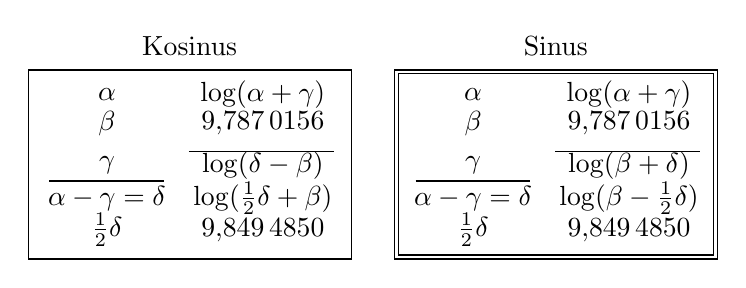
\begin{tikzpicture}[x=1cm,y=1cm]
\node at (2.05,2.55) {Kosinus};
\node at (6.70,2.55) {Sinus};
\draw (0,-.15) rectangle (4.10,2.25);
\draw (4.65,-.15) rectangle (8.75,2.25);
\draw (4.70,-.10) rectangle (8.70,2.20);
\draw (.27,.84)--(1.72,.84);
\draw (2.04,1.22)--(3.88,1.22);
\draw (4.92,.84)--(6.37,.84);
\draw (6.69,1.22)--(8.53,1.22);
\node at (1.00,1.94) {\(\alpha\)};
\node at (1.00,1.57) {\(\beta\)};
\node at (1.00,1.04) {\(\gamma\)};
\node at (1.00,.62) {\(\alpha-\gamma=\delta\)};
\node at (1.00,.22) {\(\frac12\delta\)};
\node at (2.98,1.94) {\(\log(\alpha+\gamma)\)};
\node at (2.98,1.57) {\(9{,}787\,0156\)};
\node at (2.98,1.04) {\(\log(\delta-\beta)\)};
\node at (2.98,.62) {\(\log(\frac12\delta+\beta)\)};
\node at (2.98,.22) {\(9{,}849\,4850\)};
\node at (5.65,1.94) {\(\alpha\)};
\node at (5.65,1.57) {\(\beta\)};
\node at (5.65,1.04) {\(\gamma\)};
\node at (5.65,.62) {\(\alpha-\gamma=\delta\)};
\node at (5.65,.22) {\(\frac12\delta\)};
\node at (7.63,1.94) {\(\log(\alpha+\gamma)\)};
\node at (7.63,1.57) {\(9{,}787\,0156\)};
\node at (7.63,1.04) {\(\log(\beta+\delta)\)};
\node at (7.63,.62) {\(\log(\beta-\frac12\delta)\)};
\node at (7.63,.22) {\(9{,}849\,4850\)};
\end{tikzpicture}
\end{center}
\par\noindent Das Übrige lernt man leicht auswendig.
\par\noindent\hspace*{\parindent}Wenn Sie alles herausgefunden haben, führen Sie doch einstweilen die folgenden
zwei Anwendungen aus: .\ .\ .\ .\ .
\par\medskip
\begin{center}\textsc{Gauss} an \textsc{Encke}, Göttingen, 3. März 1817.\end{center}
\par\noindent\hspace*{\parindent}.\ .\ .\ .\ .\ Vier Elemente, die Länge des Perihels, der Exzentrizitätswinkel, die Neigung
der Bahn und die Länge des Knotens, sind nun vollständig bestimmt und eingetragen. Was beim 5. Element, der Epoche der Länge, noch zu tun
ist, habe ich mir selbst vorbehalten. Beim 6., dem Logarithmus
der halben Achse, erlaube ich mir aber, Ihre Hilfe nochmals in Anspruch zu nehmen.
\par\noindent .\ .\ .\ .\ .
\clearpage
\endgroup
\end{landscape}
